\documentclass{article}
\author{2347139}

\usepackage{xcolor}
\usepackage{listings}
\usepackage[a4paper, total={6in, 8in}]{geometry}
\usepackage{graphicx}
\usepackage{tabularx}

% Define C code style
\lstdefinestyle{cstyle}{
    language=C,
    basicstyle=\ttfamily\small,
    keywordstyle=\color{blue}\bfseries,
    commentstyle=\color{green!60!black},
    stringstyle=\color{red},
    numbers=left,
    numberstyle=\tiny\color{gray},
    stepnumber=1,
    numbersep=8pt,
    backgroundcolor=\color{white},
    showspaces=false,
    showstringspaces=false,
    showtabs=false,
    frame=single,
    rulecolor=\color{black},
    tabsize=4,
    captionpos=b,
    breaklines=true,
    breakatwhitespace=false,
    escapeinside={\%*}{*)},
    morekeywords={malloc, free, printf}
}
\begin{document}
\title{Lab 2}
\maketitle

\begin{flushleft}
\large {\textbf{Implement linked list and its operations
Consider each node as structure representation of data  for your domain. Perform all operations and implement different types of linked list}}
\end{flushleft}
\section*{}
\begin{lstlisting}[style=CStyle]
    #include <stdio.h>
    // #include <conio.h>
    #include <stdlib.h>
    #include "ll.h"
    
    struct ll *head = NULL;
    
    int main()
    {
        if (head != NULL)
        {
            loop();
        }
        else
        {
            head = newll();
            loop();
        }
    }
    void loop()
    {
        int choice, pos;
        char c = 'n';
        while (1)
        {
            system("cls");
            printf("\n The List:\n");
            display(head);
            printf("\n --------------------------------");
            printf("\n \n 1. Insert In Beginning");
            printf("\n 2. Insert at End");
            printf("\n 3. Insert In Between");
            printf("\n 4. Delete");
            printf("\n \n Enter your choice:");
            scanf("%d", &choice);
            switch (choice)
            {
            case 1:
            {
                inbegin(head);
                break;
            }
            case 2:
            {
                inend(head);
                break;
            }
            case 3:
            {
                if (count(head) <= 1)
                {
                    printf("\n There is only one element in the list and can't insert inbetween");
                    break;
                }
                printf("\n Enter the position:(2-%d)", count(head));
                scanf("%d", &pos);
                inbetween(head, pos);
                break;
            }
            case 4:
            {
                del(head);
                break;
            }
            default:
            {
                printf("Invalid Input");
                break;
            }
            }
            printf("\n\n-------------------------------------------------\n Do you want to continue?(y/n)");
            scanf(" %c", &c);
            if (c == 'y' || c == 'Y')
            {
                system("cls");
            }
            else
            {
                break;
            }
        }
    }
    
    struct ll *newll()
    {
        printf("\n The List is Empty!!!!!!");
        printf("\n A new List is being created---");
        struct ll *newnode = (struct ll *)malloc(sizeof(struct ll));
        printf("\n Enter the HoneypotId:");
        fflush(stdin);
        scanf("%d", &newnode->data);
        printf("\n Enter the Honeypot Name:");
        fflush(stdin);
        scanf("%[^\n]*c", newnode->name);
        newnode->link = NULL;
        printf("\n New List created successfully");
        return newnode;
    }
    void inbegin(struct ll *temp)
    {
        struct ll *newnode = (struct ll *)malloc(sizeof(struct ll));
        printf("\n Enter the HoneypotId:");
        fflush(stdin);
        scanf("%d", &newnode->data);
        printf("\n Enter the Honeypot Name:");
        fflush(stdin);
        scanf("%[^\n]*c", newnode->name);
        newnode->link = temp;
        head = newnode;
        printf("\n Insertion at beginning is Successfull");
    }
    
    void display(struct ll *ptr)
    {
        while (ptr != NULL)
        {
            printf("%d. %s --->   ", ptr->data, ptr->name);
            ptr = ptr->link;
        }
        printf("NULL\n");
    }
    
    int count(struct ll *temp)
    {
        int count = 0;
        while (temp != NULL)
        {
            count++;
            temp = temp->link;
        }
        return count;
    }
    
    void inend(struct ll *temp)
    {
        struct ll *newnode = (struct ll *)malloc(sizeof(struct ll));
        printf("\n Enter the HoneypotId:");
        fflush(stdin);
        scanf("%d", &newnode->data);
        printf("\n Enter the Honeypot Name:");
        fflush(stdin);
        scanf("%[^\n]*c", newnode->name);
        newnode->link = NULL;
        while (temp->link != NULL)
        {
            temp = temp->link;
        }
        temp->link = newnode;
        printf("\n Insertion at End is Successfull");
    }
    
    void inbetween(struct ll *temp, int pos)
    {
        if (1 < pos <= (count(head)))
        {
            int i;
            struct ll *newnode = (struct ll *)malloc(sizeof(struct ll));
            printf("\n Enter the HoneypotId:");
            fflush(stdin);
            scanf("%d", &newnode->data);
            printf("\n Enter the Honeypot Name:");
            fflush(stdin);
            scanf("%[^\n]*c", newnode->name);
            for (i = 2; i < pos - 1; i++)
            {
                temp = temp->link;
            }
            newnode->link = temp->link;
            temp->link = newnode;
            printf("\n Insertion inbetween Completed");
        }
        else
        {
            printf("\n Invalid Position");
        }
    }
    
    void del(struct ll *temp)
    {
        printf("\n\n Enter the Emp-ID which you wish to delete:");
        int id;
        fflush(stdin);
        scanf("%d", &id);
        int pos = searchid(id);
        printf("\n The position of the node is: %d", pos);
        if (pos <= 0)
        {
            printf("\n Emp-ID doesn't exist to delete");
        }
        else if (pos == 1)
        {
            head = head->link;
            printf("\n\n Successfully removed the first node");
        }
        else if (pos == count(head))
        {
            delend(head);
            printf("\n Successfully removed the last node");
        }
        else
        {
            delbetween(head, pos);
            printf("\n Successufully removed the node");
        }
    }
    
    int searchid(int id)
    {
        int pos = 0;
        struct ll *temp;
        temp = head;
        if (id == temp->data)
        {
            pos = pos + 1;
            return pos;
        }
        else
        {
            pos++;
            while (temp != NULL)
            {
                temp = temp->link;
                pos++;
                if (id == temp->data)
                {
                    return pos;
                }
            }
        }
    }
    
    struct ll *delbegin(struct ll *temp)
    {
        struct ll *head = NULL;
        head = temp->link;
        return head;
    }
    
    void delend(struct ll *t1)
    {
        struct ll *t2;
        t2 = t1->link;
        while (t2->link != NULL)
        {
            t1 = t1->link;
            t2 = t2->link;
        }
        t1->link = NULL;
        free(t2);
    }
    
    void delbetween(struct ll *t1, int pos)
    {
        struct ll *t2;
        t2 = t1->link;
        int count = 1;
        while (count < pos - 1)
        {
            t1 = t1->link;
            t2 = t2->link;
            count++;
        }
        t1->link = t2->link;
        free(t2);
    }
    
\end{lstlisting}
\section*{Output}
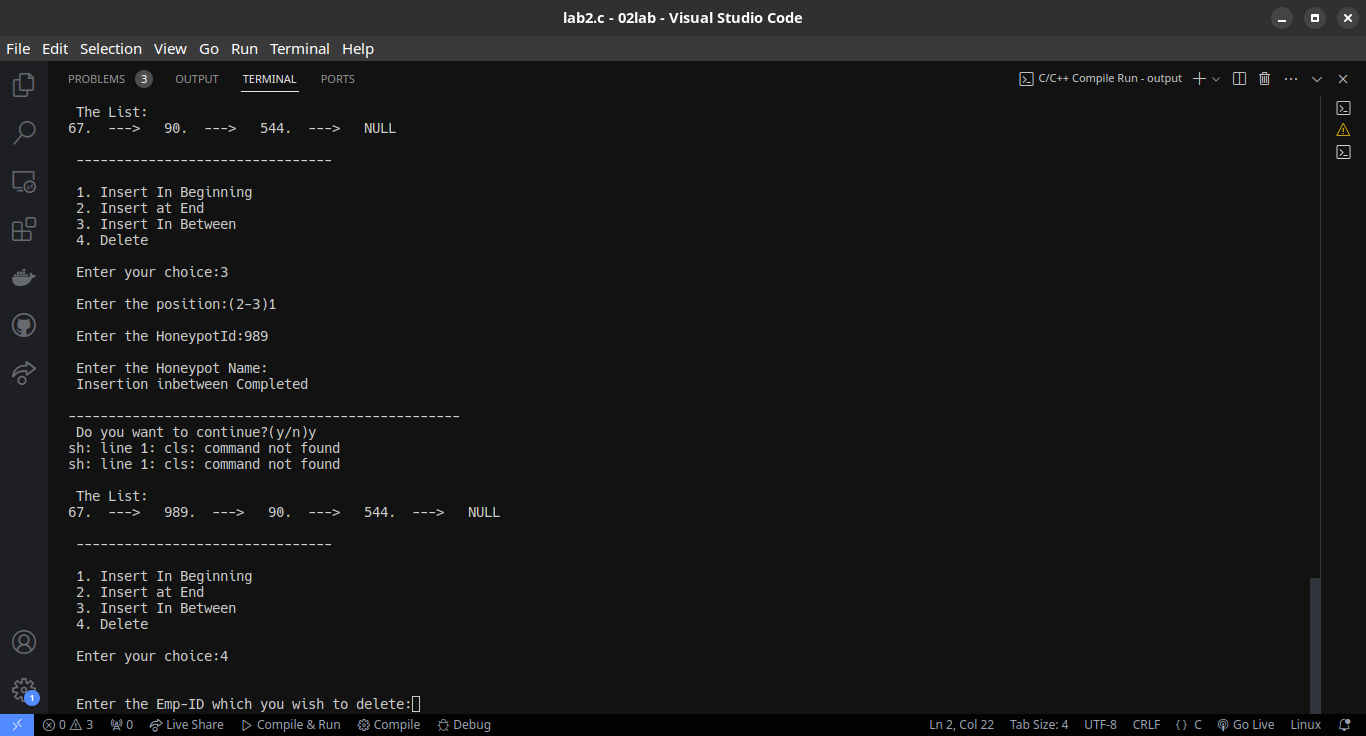
\includegraphics[width=11cm, height=9cm]{./images/01.png}
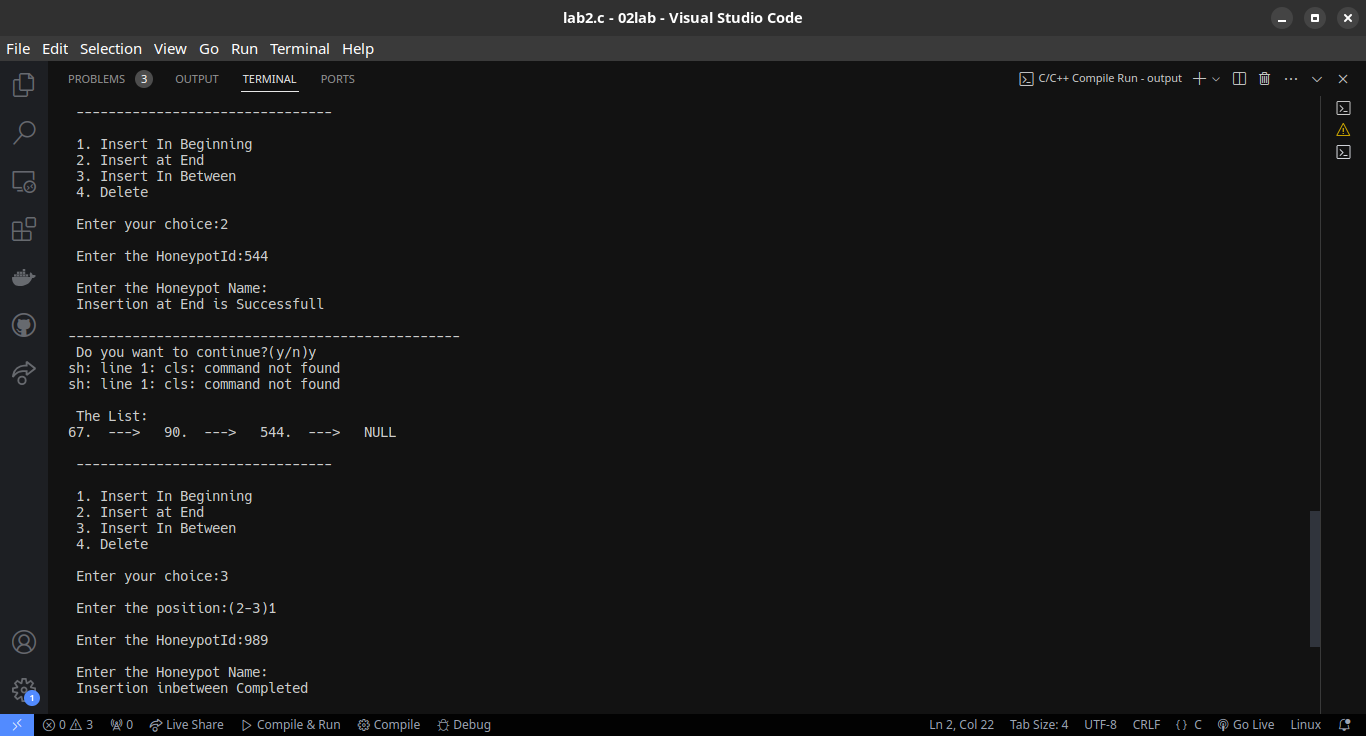
\includegraphics[width=11cm, height=9cm]{./images/02.png}
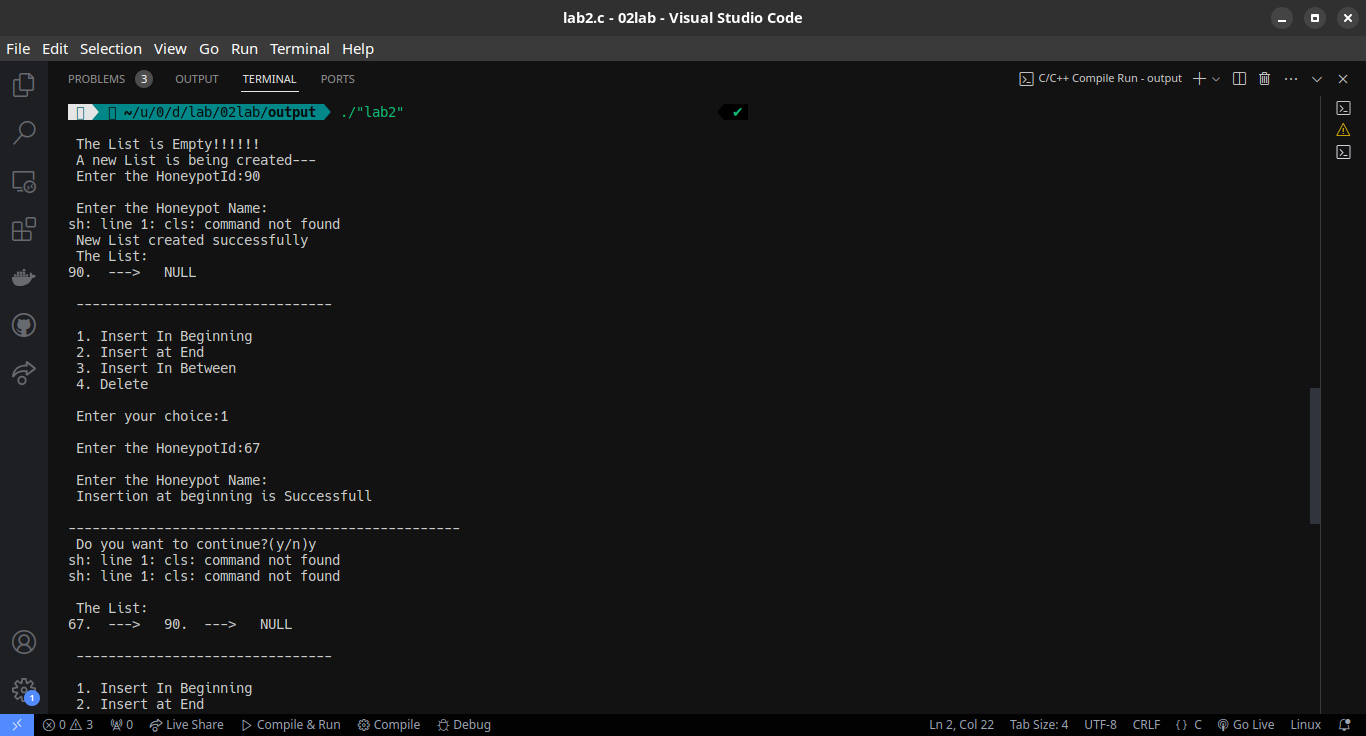
\includegraphics[width=11cm, height=9cm]{./images/03.png}



\end{document} 